\documentclass[10pt,twocolumn]{article}

\usepackage[english]{babel}
\usepackage[utf8]{inputenc}
\usepackage{mathtools}
\usepackage{graphicx}
\setlength{\marginparwidth}{2cm}
\usepackage[colorinlistoftodos]{todonotes}
\usepackage[margin=0.9in]{geometry}
\usepackage{multicol}
\usepackage[nottoc, notlof, notlot]{tocbibind}
\usepackage[backend=biber, style=authoryear]{biblatex}
\usepackage{csquotes}

\addbibresource{references.bib} % Specify the bibliography file

\title{Using Q-Learning in Sokoban: Performance Enhancements and Challenges}

\author{
  J. Tremblay\textsuperscript{1}\thanks{\texttt{jeremy-tremblay@outlook.fr}}  
  \space and T. Guyomard\textsuperscript{1}\thanks{\texttt{thomas.guyomard.pro@orange.fr}} \\
  \textsuperscript{1}Université du Littoral Côte d'Opale, Calais, France
}

\date{\today}

\begin{document}
\maketitle

\begin{abstract}
    This paper explores the application of Q-Learning to the game Sokoban, focusing on various performance enhancements and challenges encountered. Despite its simplicity, Sokoban presents significant challenges for reinforcement learning algorithms due to its complex state space and delayed rewards. We developed several versions of a Q-Learning algorithm with modifications such as wall detection, elimination of unnecessary actions, and reward system adjustments. Experimental results demonstrate varying degrees of improvement in performance with these enhancements. However, one of the primary limitations encountered was the particularly long training times required for effective learning. Our findings provide insights into the limitations and potential of Q-Learning in Sokoban, highlighting areas for future research and application.
\end{abstract}

\section{Introduction}

Reinforcement learning (RL), a branch of machine learning, has transformed how algorithms learn to make decisions by interacting with environments to maximize cumulative rewards. Among RL techniques, Q-Learning stands out for its simplicity and effectiveness in learning optimal policies through iterative trial and error.

Adapted extensively in video games, Q-Learning excels in environments where decisions influence future states and outcomes. Sokoban, a classic puzzle game where players push boxes to designated locations, presents unique challenges for reinforcement learning algorithms due to its vast state space and delayed rewards. Each action in Sokoban can have intricate consequences, making effective strategy learning challenging without extensive training and fine-tuning.

This study explores these challenges and aims to enhance Q-Learning's effectiveness in Sokoban through modifications such as wall detection, action reduction, and adjustments to the reward system. Despite advancements, a significant limitation encountered is the extended training times necessary for effective learning. These findings contribute to understanding Q-Learning in complex environments, suggesting avenues for future research and practical applications.


\section{Related Work}

Previous studies have demonstrated the effectiveness of Q-Learning and deep reinforcement learning techniques in various gaming environments. Mnih et al. (2013) \cite{mnih2013playing} pioneered the use of deep Q-Learning to learn game policies directly from pixel inputs, achieving human-level performance on multiple classic Atari games.

In the realm of real-time strategy games, Vinyals et al. (2019) \cite{vinyals2019grandmaster} showcased advanced Q-Learning and reinforcement learning methods in achieving Grandmaster level performance in StarCraft II. Their work exemplifies the application of sophisticated learning algorithms to master complex strategic environments.

These studies highlight the versatility of Q-Learning in adapting to diverse gaming dynamics, from classic Atari games to complex real-time strategy scenarios like StarCraft II. In contrast, the challenges specific to Sokoban, such as sparse rewards and intricate state transitions, remain less explored although we can cite the work of Sébastien Racanière et al. (2017) \cite{racaniere2017imagination} on the subject of reinforcement learning. This study aims to address these challenges in puzzle-solving domains.

\section{Theoretical Foundations}

\subsection{Q-Learning Basics}

Q-Learning is a reinforcement learning technique used to learn optimal actions to take in a given state to maximize cumulative rewards. At its core, Q-Learning maintains a Q-Table (or Q-Function), denoted as \( Q(s, a) \), where \( s \) represents a state and \( a \) an action. The table is updated iteratively based on the Bellman equation:

\[
    Q(s, a) \leftarrow (1 - \alpha) \cdot Q(s, a) + \alpha \cdot \left( r + \gamma \cdot \max_{a'} Q(s', a') \right)
\]

Here, \\
- \( \alpha \) (learning rate) controls how much new information overrides old information. \\
- \( \gamma \) (discount factor) determines the importance of future rewards. \\
- \( r \) is the immediate reward received after taking action \( a \) in state \( s \). \\
- \( s' \) is the resulting state after taking action \( a \). \\

The Q-Table stores the expected future rewards for all state-action pairs, guiding the agent's decision-making process during exploration and exploitation phases.

\subsection{Exploration-Exploitation Trade-off}

In Q-Learning, \( \epsilon \) controls the exploration-exploitation trade-off, crucial for learning optimal strategies in dynamic environments. The \( \epsilon \)-greedy policy dictates action selection:

\[
    \pi(a|s) =
    \begin{cases}
        1 - \epsilon + \frac{\epsilon}{|\mathcal{A}(s)|}, & \text{if } a = \arg\max_{a'} Q(s, a') \\
        \frac{\epsilon}{|\mathcal{A}(s)|},                & \text{otherwise}
    \end{cases}
\]

Here, \( Q(s, a) \) denotes the Q-value of action \( a \) in state \( s \), \( \mathcal{A}(s) \) represents the set of possible actions in state \( s \), and \( |\mathcal{A}(s)| \) is the number of actions available in state \( s \).

Initially set high (e.g., 1.0), \( \epsilon \) encourages exploration early in training. As training progresses, \( \epsilon \) is generally reduced to prioritize exploitation of learned actions.

\subsection{Implementation Details}

In our implementation, we focused on guiding the agent's behavior through a carefully designed reward system. The system was crucial in reinforcing desired actions, such as pushing boxes onto targets, while discouraging undesired actions like pushing boxes off targets. These rewards were iteratively adjusted to improve the agent's learning process and performance in solving the Sokoban puzzle efficiently.

State representation involved converting the Sokoban map into a numerical format to ensure state uniqueness and reduce complexity. This approach facilitated effective learning and decision-making by the Q-Learning algorithm.
\section{Methodology}

\subsection{Tools}

The implementation was conducted using the Python programming language, leveraging the Gym Sokoban \cite{SchraderSokoban2018} library. Gym Sokoban provides a simulated environment for the Sokoban game, facilitating the integration of reinforcement learning algorithms for experimentation and evaluation.

\subsection{Initialization of Q-Learning}

To evaluate the effectiveness of Q-Learning in the Sokoban game context, we began by implementing a basic Q-Learning algorithm using the Gym Sokoban library in Python. The Q-Table was initialized with default parameters ($\alpha$ = 0.5, $\gamma$ = 0.95, $\epsilon$ = 0.1).

\subsection{Reward System}

The initial reward system was defined as follows:
\begin{itemize}
    \item Performing an action: -0.1
    \item Pushing a box onto a target: +1.0
    \item Pushing a box off a target: -1.0
    \item All boxes on targets: +10.0
\end{itemize}

\subsection{State Representation}

To ensure state uniqueness, we converted the Sokoban map into a numerical representation and hashed it to obtain a unique state identifier. This approach reduced state complexity while preserving uniqueness.

\subsection{Iterative Improvements}

We introduced several modifications to enhance Q-Learning performance:
\begin{itemize}
    \item Detection of losing conditions to avoid ineffective actions.
    \item Restriction of the "do nothing" action to promote active movements.
    \item Optimization of alpha, gamma, and epsilon parameters, as well as the reward system, to improve learning.
\end{itemize}

\subsection{Generalization Evaluation}

We evaluated the model's ability to generalize to new Sokoban levels by testing its performance without complete retraining. This methodology enabled us to explore the capabilities and limitations of Q-Learning in a complex gaming environment.

\section{Implementation and Results}

\subsection{Initial Q-Learning Implementation}

We began by implementing Q-Learning on a Sokoban puzzle with three boxes using the Gym Sokoban library in Python. The chosen level (Figure \ref{fig:sokoban_level}) is a representative example of Sokoban's complexity, where the agent must strategically move three boxes to designated target locations.

\begin{figure}[ht]
    \centering
    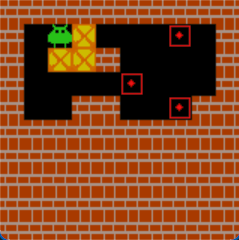
\includegraphics[width=0.3\textwidth]{Images/sokoban.png}
    \caption{Example Sokoban level used for these Q-Learning experiments.}
    \label{fig:sokoban_level}
\end{figure}

Initially, the Q-Learning agent struggled to solve the puzzle, requiring approximately 1630 episodes to achieve its first successful completion. After this initial breakthrough, the agent demonstrated improved learning efficiency, achieving successful completions in subsequent attempts. This performance is described in (Figure \ref{fig:initial_results}).

\begin{figure}[ht]
    \centering
    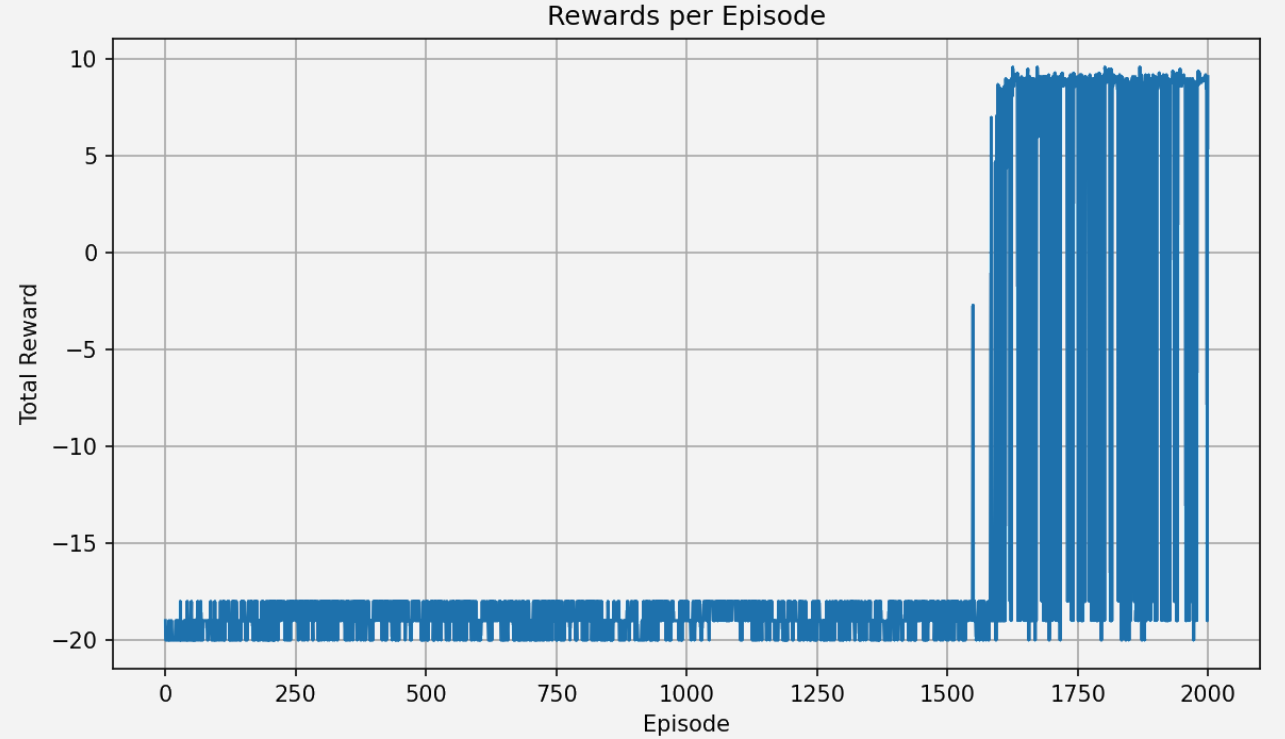
\includegraphics[width=0.49\textwidth]{Images/resultats_initial.png}
    \caption{Initial results of the Q-Learning algorithm on the Sokoban puzzle.}
    \label{fig:initial_results}
\end{figure}

This figure shows the average reward per episode for a game of Sokoban. For each simulation, we decided to launch 2000 games to see the results, because we think this amount is relevant to determine if the agent performs correctly or not. Initial fluctuations indicate inconsistency, but after the first successful solve (which can be seen with the sudden peak in rewards), rewards stabilize, reflecting improved performance and more frequent wins.

It is also important to note that the execution time for these experiments was relatively long, with each episode taking approximately 1.5 seconds to complete. This extended training time is a significant limitation of the Q-Learning algorithm in complex environments like Sokoban.

\subsection{Loss Detection and Penalty}

To improve the agent's performance, we implemented a loss detection mechanism to identify and penalize unsolvable states.

First, we identified three scenarios that could lead to a loss:
\begin{enumerate}
    \item A box is stuck in a corner.
    \item A box is trapped between other boxes but can still be moved if others are shifted.
    \item No boxes appear stuck, but the overall configuration makes the level unsolvable.
\end{enumerate}

We focused on detecting the first case, where a box is irreversibly stuck in a corner.

The following pseudo-code illustrates the algorithm for detecting when a box is stuck in a corner:

\begin{verbatim}
for each box in boxes:
    if box is in a corner:
        terminate episode
        apply penalty of -10 points
\end{verbatim}

Implementing this detection and penalty improved the agent's performance, as shown in Figure \ref{fig:performance_wall_detection}. The agent was able to avoid dead-end situations more effectively, reducing the number of futile episodes and improving the overall learning efficiency.

\begin{figure}[ht]
    \centering
    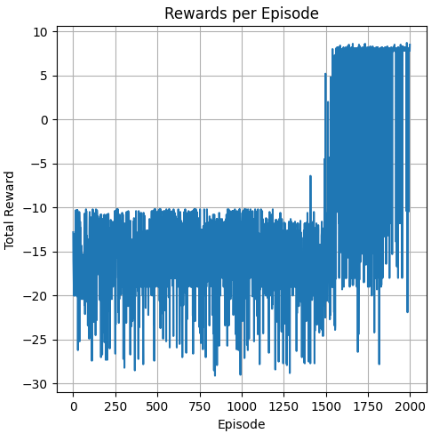
\includegraphics[width=0.49\textwidth,height=6cm]{Images/performance_wall_detection.png}
    \caption{Performance improvement with loss detection and penalty for boxes stuck in corners.}
    \label{fig:performance_wall_detection}
\end{figure}

From this figure, we observe more variations in rewards, which result from penalizing the agent when the game is in a loss state. The agent found the optimal path more quickly, around 1500 episodes. The execution time has also been reduced to 1.3 seconds per episode due to this improvement.

This improvement helps the agent recognize when it is making mistakes and learn from them.

\subsection{Removing No-Op Action}

To further enhance the agent's performance, we decided to address situations that led to unnecessary actions. We have decided to keep the previous improvements.

In the game of Sokoban, there are several possible actions: moving in each of the four directions and pushing a box in each of the four directions, making a total of eight actions. Additionally, there exists an action where the agent does nothing, which can be likened to a human "thinking." However, in the context of AI, this action is redundant as we aim to minimize execution time. We noticed that around 20\% of the actions taken by our model in the previous simulation were this one. To refine the agent's behavior further, we removed the "no-op" (no operation) action, which did not contribute to solving the puzzle.

The impact of this modification is shown in Figure \ref{fig:performance_no_op}. Although the improvement was marginal, the agent's performance showed a slight increase in the number of successful episodes, and it started finding the optimal path around 1400 episodes.

\begin{figure}[ht]
    \centering
    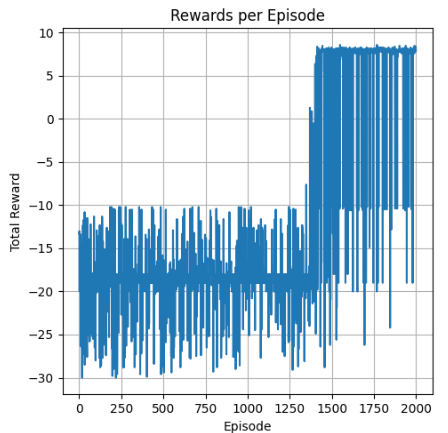
\includegraphics[width=0.49\textwidth,height=6cm]{Images/performance_no_op.png}
    \caption{Performance after removing the no-op action.}
    \label{fig:performance_no_op}
\end{figure}

\subsection{Penalizing Invalid Moves}

Building on the previous improvement, we introduced a penalty system to discourage the agent from making invalid moves, such as attempting to push a box where there is none or moving into walls. The objective was to enhance the agent's decision-making by penalizing ineffective actions and guiding it towards more productive strategies.

The penalty for these invalid moves was set to -0.5 points. However, during our experiments, we observed that the agent was unable to finish the level at all, even once in 2000 episodes, regardless of the penalty value. We think that this excessive penalization led to a decline in performance. The agent became overly cautious, resulting in reduced exploration and an overall negative impact on its ability to solve the puzzle efficiently. Furthermore, this method felt somewhat like guiding our agent through the level.

This suggests that while discouraging invalid moves is important, excessive penalties can hinder the learning process. Therefore, this approach was ultimately deemed counterproductive and was abandoned in favor of other methods.

\subsection{Parameter Tuning}

To optimize the Q-Learning performance, we experimented with tuning the algorithm's parameters: $\alpha$ (learning rate), $\gamma$ (discount factor), and $\epsilon$ (exploration rate). The default values used were $\alpha = 0.5$, $\gamma = 0.95$, and $\epsilon = 0.1$. After a random search, we did not observe any remarkable difference between the parameter values. Additionally, we attempted to fine-tune the reward system parameters to better guide the agent's learning process.

The parameter tuning process involved using an optimization algorithm (search tree) to find the best combination of values. However, this process proved to be computationally expensive and time-consuming. After 16 hours of optimization with a very small number of iterations (20 trials of 2000 steps), the settled parameters were:

\begin{itemize}
    \item Correct box placement: 8
    \item Invalid box placement: 0
    \item Victory: 0
    \item Defeat: -7
    \item Step penalty: -0.14972124706419776
\end{itemize}

At first glance, the results are surprising, but we trained an agent with these settings. Despite these efforts, the results were not as expected. The agent learned to exploit the reward system by repeatedly moving boxes back and forth to gain points without solving the puzzle. This behavior highlighted the difficulty in balancing reward structures and parameter values in Q-Learning.

We think that an execution time of 1.3 seconds per episode is too long to simulate many episodes and find the best parameters. We need to find a way to reduce this time to be able to find the best parameters, such as rewriting the code in a faster language like C++.

\subsection{Generalization Issues}

After these unsuccessful attempts, we tested the agent's ability to generalize to new Sokoban levels without complete retraining. To do this, we reused the Q-table extracted from the previous best trainings and placed the agent on a new level with the same number of boxes. The agent was unable to solve the puzzle efficiently, requiring over 1700 episodes to start solving the puzzle, worse than the initial learning phase.

This experience indicated that the state representation, tied to the entire map, was too specific and did not promote generalization. We think a better approach would be to use a more general state representation that can be used on different levels, such as representing only a 5x5 square around the agent. This would allow the agent to generalize its learning to different levels, even though finding the optimal path could be more challenging. Another solution would be to represent only the boxes, targets, and the agent, omitting the walls. There are many possibilities, and we think a mix of approaches could yield good results, offering a path for future research.

We then deeply investigated whether we could consider our model "stable" once it had learned to solve the puzzle. We wanted to check if it made many mistakes even after successfully completing the level in the past. We reported the number of games won and lost after the first victory on the same level to observe changes. Figure \ref{fig:number_of_game_won} shows the results of this experiment.

\begin{figure}[ht]
    \centering
    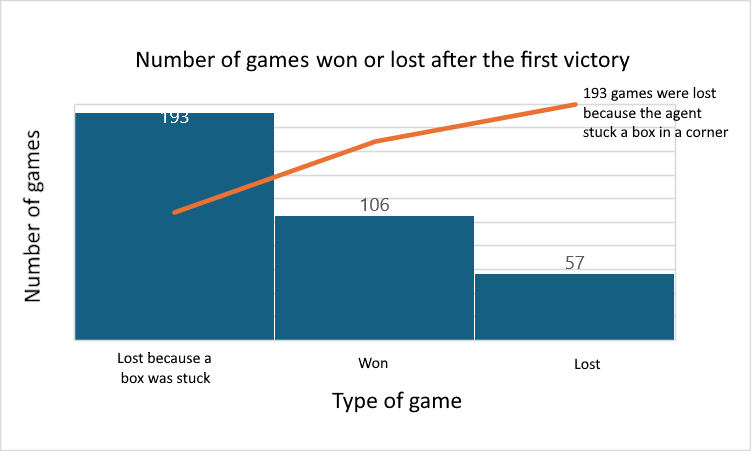
\includegraphics[width=0.49\textwidth]{Images/number_of_game_won.png}
    \caption{Number of endgame types after first win.}
    \label{fig:number_of_game_won}
\end{figure}

The first bar in the figure shows the games lost and ended by our program, where the agent stuck a box in a corner. The second bar represents the number of games won by the agent, and the last bar shows the games lost by the agent (after 200 iterations). We can see that the agent finishes the level about 2 times out of 7.

We observe that the agent is not stable at all; it has difficulty solving the puzzle even after the first successful game. We think we can address this issue by using a decreasing epsilon to make the agent explore more at the beginning and exploit more when it has already learned the optimal path.

\section{Discussion}

In conclusion, our study demonstrates the challenges and potential of applying Q-Learning to the game of Sokoban. Despite various modifications, including end-game detection, action refinement, and parameter tuning, the performance improvements were limited and highlighted significant areas for further research.

Future work should focus on optimizing the code for faster execution, enabling more extensive parameter tuning without prohibitive computational costs. Additionally, comparing Q-Learning with other models such as Monte Carlo Tree Search (MCTS) and Deep Q-Learning (DQL) could provide valuable insights into more efficient learning strategies.

Finally, exploring smaller state representations could help improve the agent's ability to generalize across different levels. By addressing these aspects, we can enhance the effectiveness of reinforcement learning algorithms in complex environments like Sokoban.

\printbibliography

\end{document}